\chapter{Future Work}
\chaptermark{Future Work}
\label{ch:futurework}

%\section{Introduction (Need to rewrite)}
%\label{sec:Introduction}


Smart contracts are computer programs running atop blockchain platforms to manage large sums of
money, carry out transactions of assets, and govern the transfer of digital rights between multiple
parties.
Ethereum~\cite{Ethereum} and EOS~\cite{EOS} are among the most popular blockchain platforms which
support smart contracts and have them applied in many areas, such as finance, supply chain,
identity management, games, etc.
As of April 2021, there are over XXX smart contracts deployed on Ethereum, which is a XXX fold
increase since just two years ago~\cite{Etherscan}.
These smart contracts have enabled about 3.1 K decentralized applications (DApps) serving 80 K
daily users.
%\todo[inline]{talk about contract security.}


Smart contracts deployed on permissionless blockchains, such as Ethereum, are accessible to any
user in a trust-less environment.
Therefore, most smart contract applications implement access control policies to protect their
valuable assets from unauthorized accesses.
The correctness of such policies is critical for maintaining smart contract security.
For example, suicidal contracts~\cite{nikolic2018finding} is a class of vulnerable smart contracts
without proper access control to the ``\texttt{selfdestruct}'' operations, which appear in around
20\% of unique smart contracts~\cite{oyente}.
Another high-profile victim due to vulnerable access control policy is the Parity Wallet.
The wallet was hacked through two different attack vectors resulting in the stolen of \$30M USD and
the frozen of \$100M USD, respectively.
The Parity Wallet consumes a library contract, called WalletLibrary, to implement the basic
functionality of a wallet.
Anybody can deposit money into the wallet, but only the contract owner can withdraw the funds.
The first attack vector exploited the unprotected initialization function to set the attacker as
the contract owner and finally withdrew a large sum of money deposited by other wallet users.
The root cause of this attack is that an unauthorized user can bypass the contract rule rather than
the intended user access.

A difficulty in validating the conformance to such policies, i.e., whether the contract
implementation adheres to the expected behaviors, is the lack of policy specifications. The
current practice is to implement intended access control policies with ad-hoc
Solidity~\cite{solidity} (i.e., the programming languages used to develop Ethereum smart contracts)
idioms, such as the ``\texttt{require}''statements, to check if the address of a user is in a
predefined whitelist.
Many security vulnerabilities mentioned earlier are results from this ad-hoc approach.
In particular, when the number of roles and the complexity of access patterns increase, it becomes
fairly easy for contract developers to make mistakes and introduce bugs causing security
vulnerabilities.

\begin{figure}[t]
	\centering
	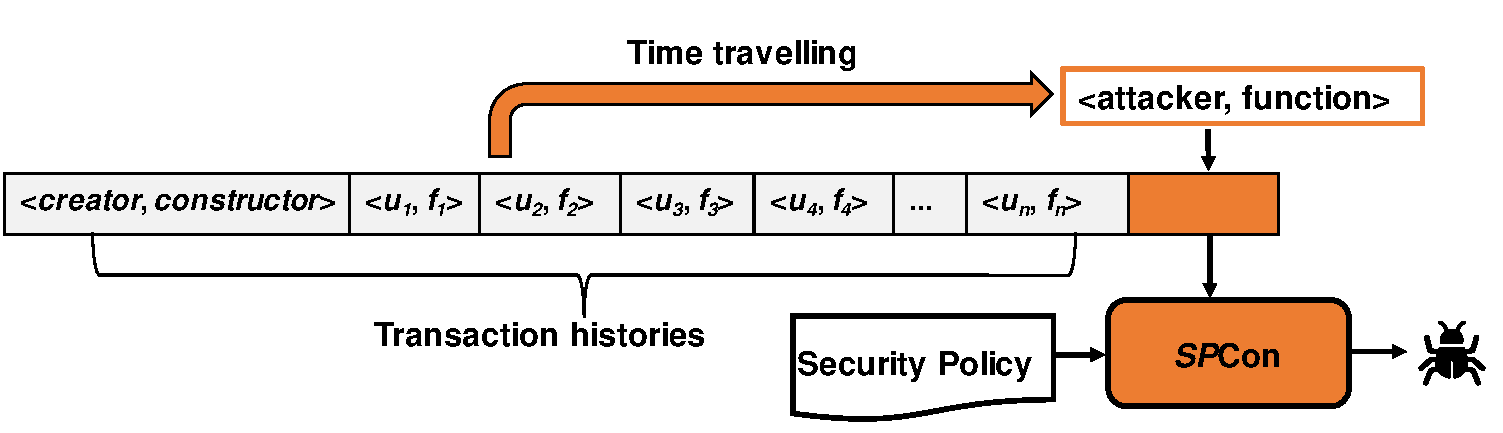
\includegraphics[width=\linewidth]{Figures/Chapter4/SPconIllustration-crop.pdf}
	\caption{Illustration of the time-travel-based security policy validation.}
	\label{fig:time-travel}
\end{figure}

In this paper, we would like to address this problem by relying on past transactions of a contract
to recover a \emph{likely} access control model, which can then be validated against various
security rules and identify potential bugs related to user permissions.
We plan to implement a security policy validator powered by ``time traveling'' through transaction
histories.
As is shown in \cref{fig:time-travel}, the key idea is that, because of the transparency and
immutability of blockchain transactions, the transaction histories of a smart contract application
from its initial deployment up to today are always available on the blockchain.
The historical transactions of a smart contract contain benign user behaviors, assuming the
contract is not yet attacked by any malicious party.
Due to the unique nature of DApps, we can safely assume that the history of a smart contract is
\emph{clean}, if it is still \emph{alive}, i.e., not being destructed or abandoned.
Therefore, we are able to reverse engineer an access control model which is permissible enough to
subsume all historical transactions.
Since historical transactions only under-approximate the behaviors allowed by the contract
implementation, by validating the recovered model against the actual contract implementation, we
will be able to discover discrepancies, indicating potential future violations of security policies.